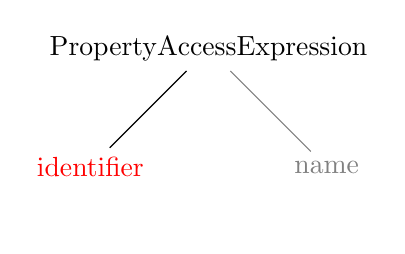
\begin{tikzpicture}
	\node {PropertyAccessExpression}
		child {node [red] {identifier}}
		child [white] {node [yshift = -0.5cm] {\phantom{node}}}  % ensure same height as sibling figures
		child [gray] {node [gray] {name}}
		;
\end{tikzpicture}
\caption[LoF entry]{
	Node pattern for a JavaScript property access, such as in:

	\code{\lowlight{return }\uline{\lowlight{obj}.\highlight{prop}}\lowlight{;}}
}
